% !TeX spellcheck = en_GB

% ------------------------------- %
%% Random Forest Classifier %%
% ------------------------------- %

\begin{frame}{Random Forest for Classification}

{\small Package \texttt{\{randomForest\}}\vspace{-1.5ex}
\begin{itemize}\setlength{\itemsep}{-0.5ex}
	\item \lstinline|randomForest(formula, data=NULL, ntree=500, mtry=sqrt(p), importance=TRUE,|\texttt{\dots)}
	\item \lstinline|importance(x, type=NULL, class=NULL,|\texttt{\dots)}
    \item \lstinline|varImpPlot(x, sort=TRUE,|\texttt{\dots)}
    \item \texttt{x\$confusion}
    \item \texttt{x\$err.rate}
\end{itemize}}

{\texttt{x}} is a {\texttt{randomForest}} object;

{\texttt{ntree}} = number of trees grown;

{\texttt{p}} = number of predictors;

{\texttt{mtry}} = number of predictors sampled for splitting at each node.

\end{frame}

% ------------------------------- %

\begin{frame}{OOB Error}
\begin{columns}
\begin{column}{0.35\textwidth}

{\footnotesize \begin{itemize}
	\item $p$ = 8
	\item \texttt{mtry} = $\sqrt{p} \simeq 3$
	\item \texttt{ntree} = 500
	\item OOB estimate error rate: $24.41\%$
\end{itemize}}

\vspace{0.5cm}

\; Model selection:
{\footnotesize \begin{itemize}
	\item \texttt{ntree} = 111
	\item min OOB error rate = 0.2343
\end{itemize}}

\end{column}
\begin{column}{0.75\textwidth}
\begin{figure}
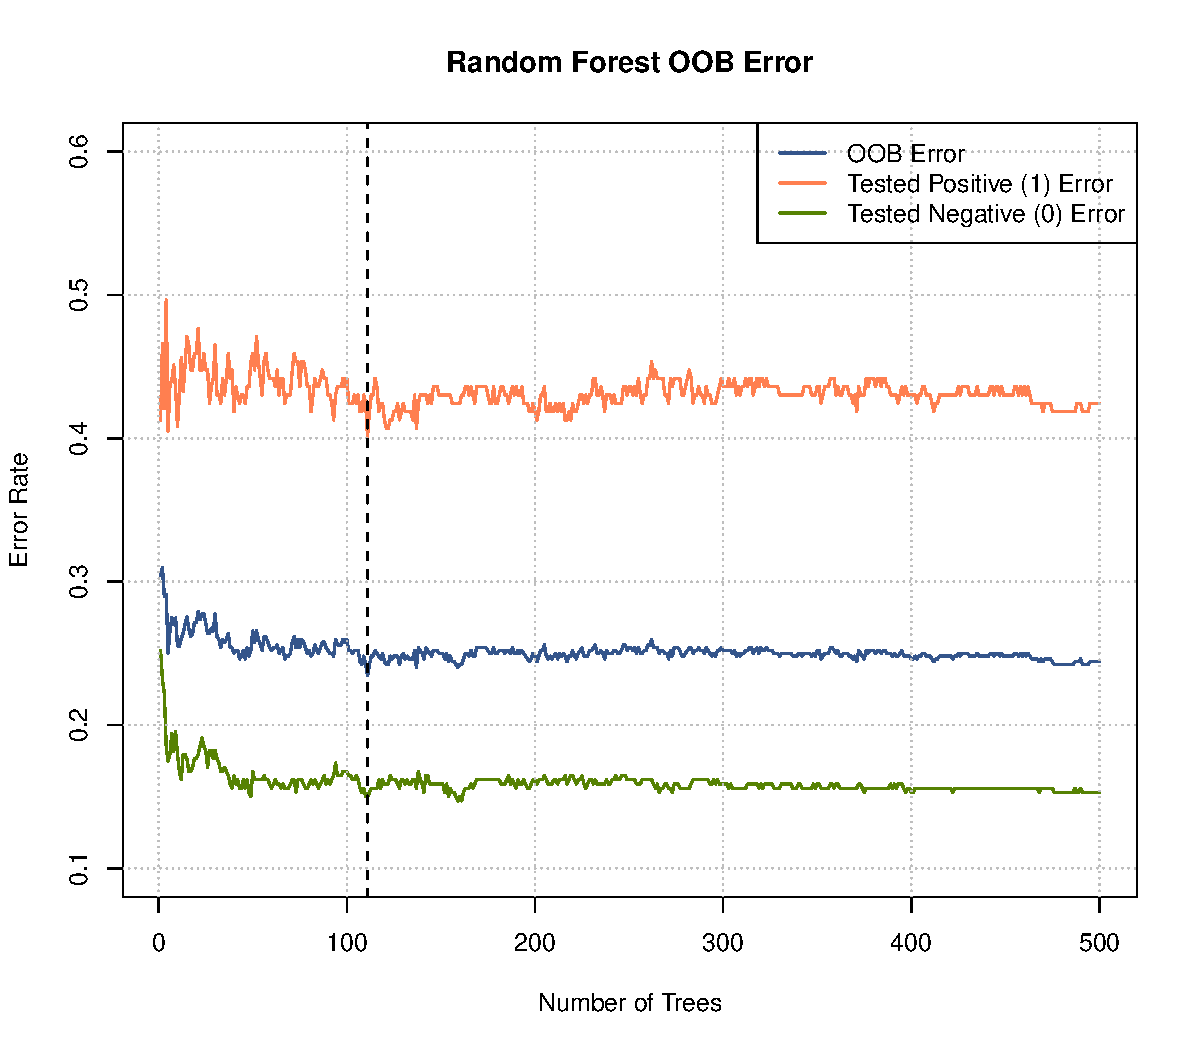
\includegraphics[width=1.05\columnwidth]{./Figures/forest/diabete_forest_error3.pdf}
\end{figure}
\end{column}
\end{columns}
\end{frame}

% ------------------------------- %

\begin{frame}{OOB Error}

\begin{columns}
\begin{column}{0.35\textwidth}
{\footnotesize \begin{itemize}
	\item $p$ = 8
	\item \texttt{mtry} = 4 
	\item \texttt{ntree} = 500
	\item OOB estimate error rate: $25\%$
\end{itemize}}

\vspace{0.5cm}

\; Model selection:
{\footnotesize \begin{itemize}
	\item \texttt{ntree} = 136
	\item min OOB error rate = 0.2226
\end{itemize}}

\end{column}
\begin{column}{0.75\textwidth}
\begin{figure}
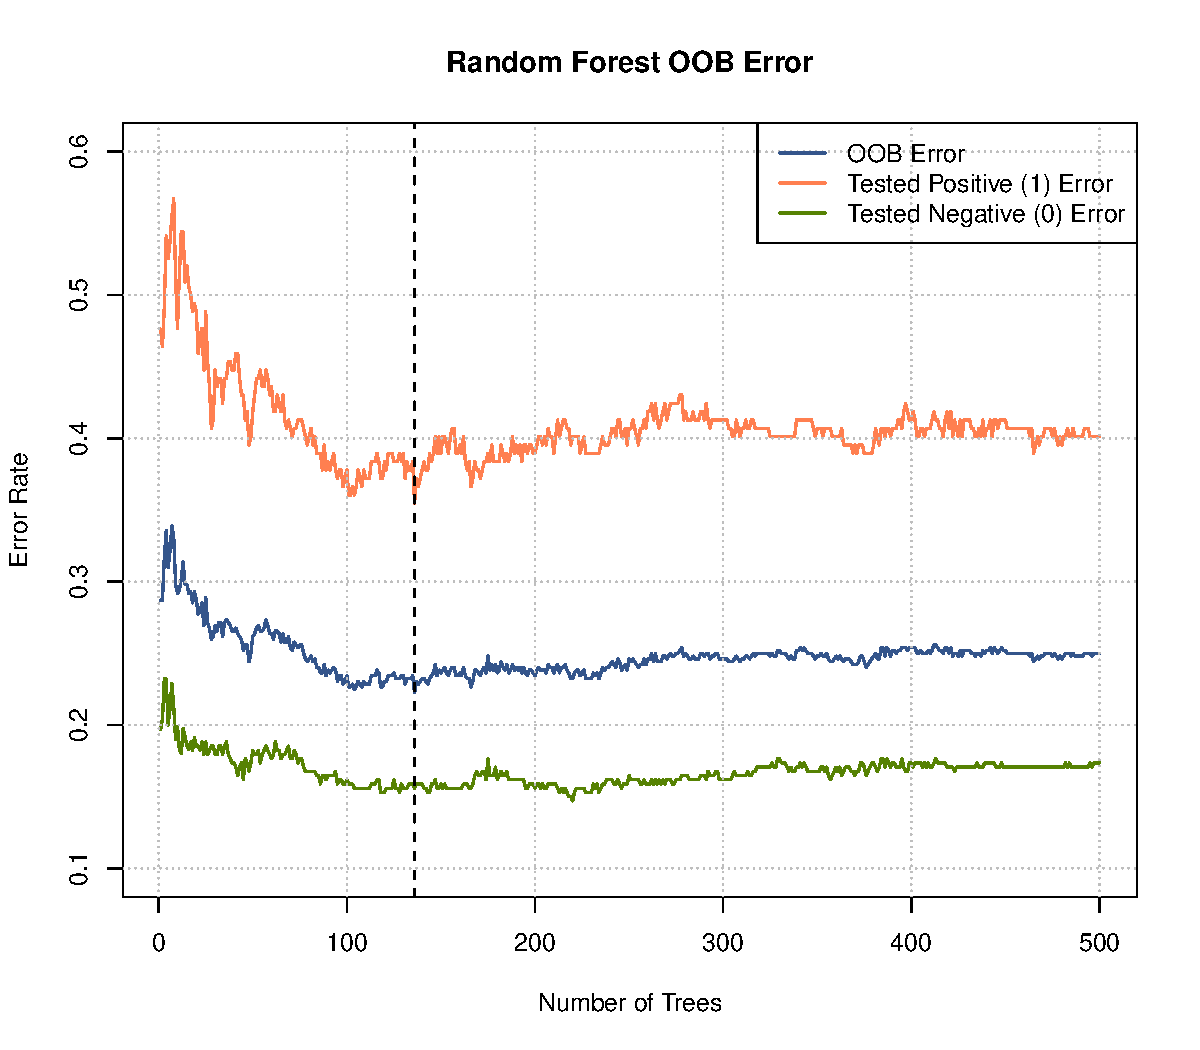
\includegraphics[width=1.05\columnwidth]{./Figures/forest/diabete_forest_error4.pdf}
\end{figure}
\end{column}
\end{columns}

\end{frame}

% ------------------------------- %

\begin{frame}%{Variable Importance}

\begin{figure}
\hspace*{-1.5em}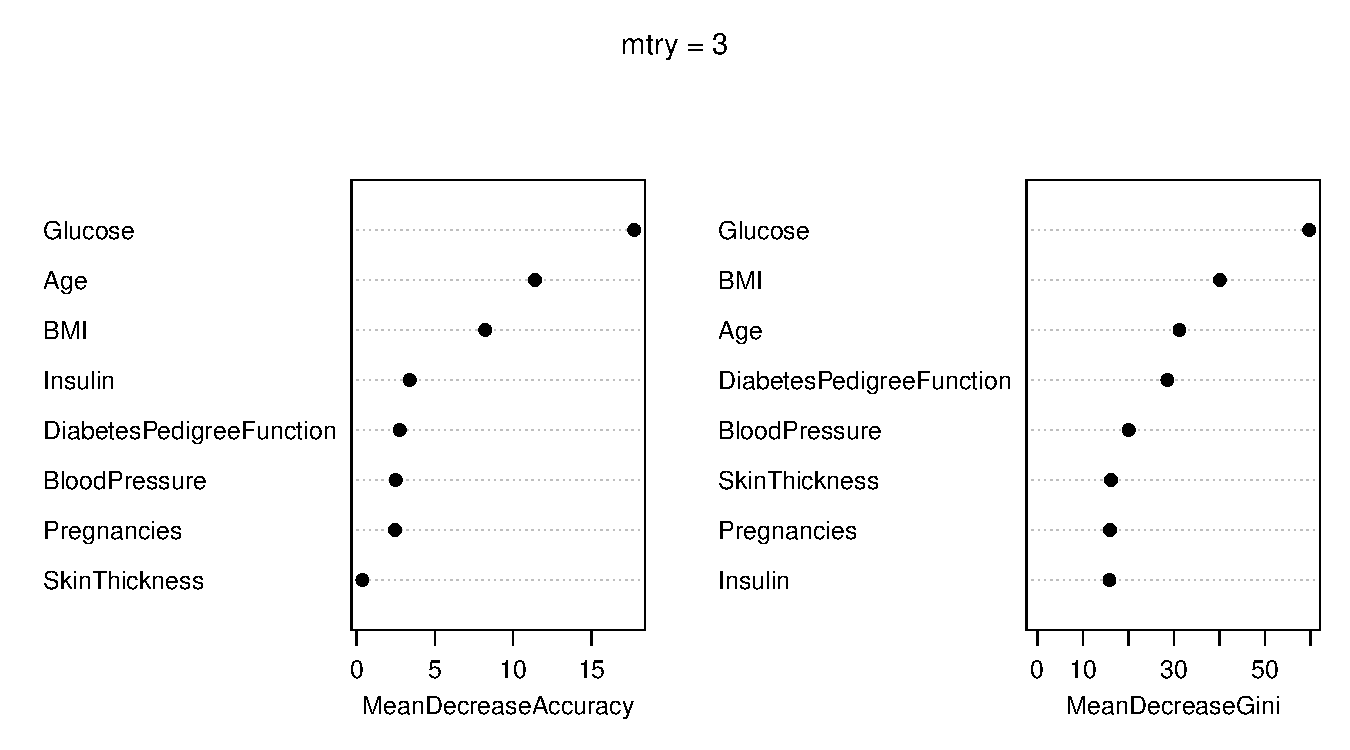
\includegraphics[width=0.78\textwidth]{./Figures/forest/diabete_var_imp3.pdf}
\hspace*{-1.5em}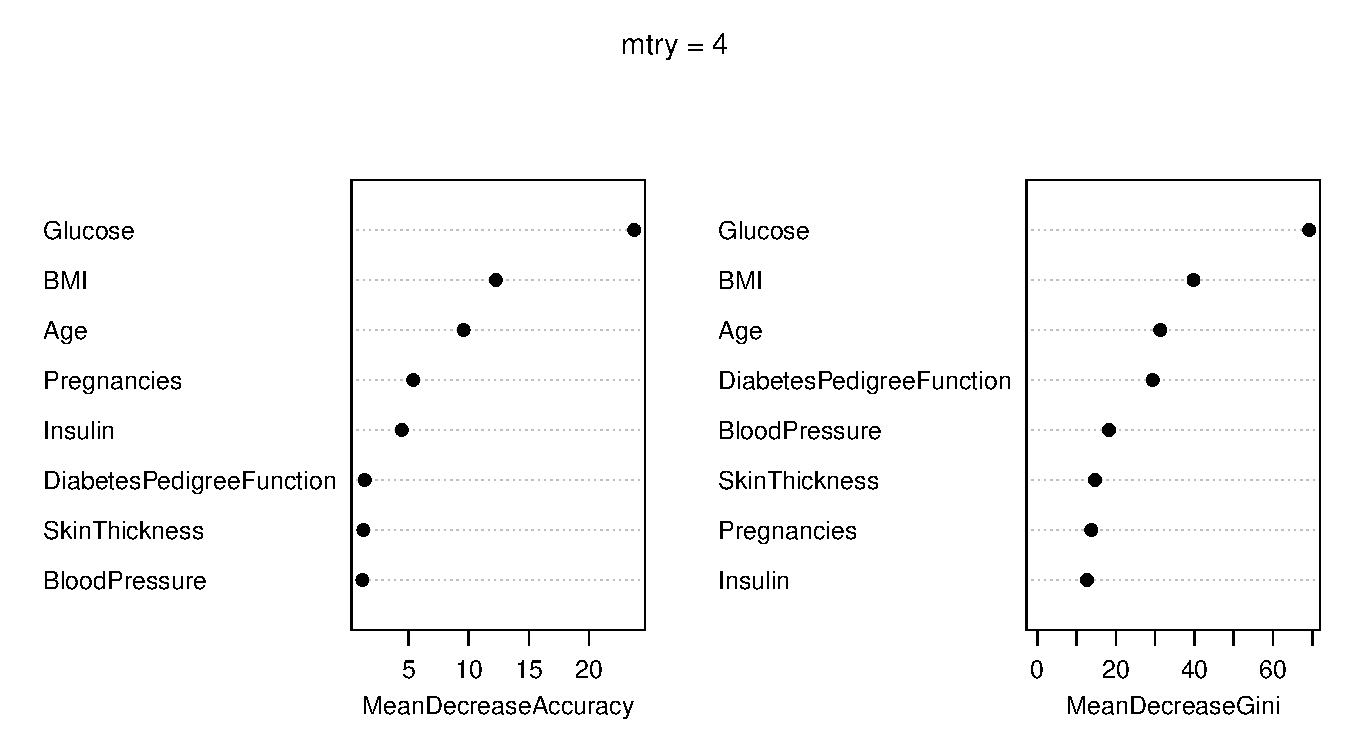
\includegraphics[width=0.78\textwidth]{./Figures/forest/diabete_var_imp4.pdf}
\end{figure}
\end{frame}

% ------------------------------- %
